% various abbreviations
\renewcommand{\L}{{\mathscr{L}}}
\newcommand{\MSbar}{$\overline{\mathrm{MS}}$}
\newcommand{\BR}{{\text{BR}}}
\newcommand{\LO}{{\text{LO}}}
\newcommand{\NLO}{{\text{NLO}}}
\newcommand{\EW}{{\text{EW}}}
\newcommand{\QCD}{{\text{QCD}}}
\newcommand{\QED}{{\text{QED}}}
\newcommand{\LEP}{{\text{LEP}}}
\newcommand{\SLD}{{\text{SLD}}}

\newcommand{\SM}{{\text{SM}}}
\newcommand{\PH}{\text{Higgs}}
\newcommand{\YM}{{\text{YM}}}
\newcommand{\Yuk}{{\text{Yukawa}}}
\newcommand{\ferm}{{\text{Matter}}}
\newcommand{\Born}{{\text{Born}}}
\newcommand{\born}{{\text{Born}}}
\newcommand{\corr}{{\text{corr}}}
\newcommand{\onel}{{\mbox{\scriptsize 1-loop}}}
\newcommand{\weak}{{\text{weak}}}
\newcommand{\gs}{g_{s}}
\newcommand{\alphas}{\alpha_{s}}
\newcommand{\muF}{\mu_{F}}
\newcommand{\muR}{\mu_{R}}
\newcommand{\sw}{\sin \theta_W}
\newcommand{\cw}{\cos \theta_W}
\newcommand{\GF}{G_\mu}

\newcommand{\Pl}{\ell}
% roman symbols
\newcommand{\rc}{{\mathrm{c}}}
\newcommand{\rI}{{\mathrm{I}}}
\newcommand{\ri}{{\mathrm{i}}}
\newcommand{\rd}{{\mathrm{d}}}
\newcommand{\rU}{{\mathrm{U}}}
\newcommand{\rL}{{\mathrm{L}}}
\newcommand{\rR}{{\mathrm{R}}}
\newcommand{\rT}{{\mathrm{T}}}
\newcommand{\rY}{{\mathrm{Y}}}

%In the first part of this chapter, we give a brief introduction to the \SM~(SM), which forms
%the theoretical basis of the work described in this thesis. The second
%half gives a short introduction into the phenomenology of hadron
%colliders.

%In the following, we describe several aspects of the theory background of the
%SM. In particular, we aim at illustrating the concepts of gauge
%invariance and spontaneous symmetry breaking.

In this chapter, we give a very brief overview of the theoretical framework
for the work presented in this thesis, as well as the basic notions we
will operate with in the following chapters.
For any details regarding the content of this chapter we refer to many excellent textbooks, such as \cite{PeskinS,Schwartz:2013pla}.


\section{The Standard Model}

The \emph{Standard Model} of particle physics (SM) is the best known unified description of three of the
four known fundamental forces: electromagnetism, weak, and strong.
Together with the General Relativity as a theory of gravity,
they describe the majority of observed phenomena of nature.

The SM is a local quantum field theory (QFT) formulated on a flat background Minkowski space-time in $3+1$ dimensions.
As such, it's properties are described by the \emph{action}
\[
  S = \int \dd[4]{x}~\L(x),
\]
with the \emph{Lagrangian} $\L$. 
In the context of quantum theory, the correlation functions
are obtained as integrals over all field configurations, to which the action assigns phases.
The invariance under translations and rotations in space-time is built in the theory as the
invariance of its action under the transformations of the Poincaré group.
Each fundamental particle is associated to a quantum field.
The fields are classified according to irreducible representations of the Poincaré group,
which determine their kinematical properties, such as spin and statistics.


Schematically, the Lagrangian of the SM can split into four sectors,
\begin{equation}
  \L_\SM = \L_\YM + \L_\ferm + \L_\PH + \L_\Yuk,
\end{equation}
and we will briefly discuss each of them in this section.

\subsection{Gauge Structure}
\label{sec:giym}

The interactions of particles are realized as local gauge symmetries of the action (or the Lagrangian).
In particular, the gauge group of the SM is
\begin{align}\label{eq:SMgauge}
  SU(3)_C\otimes SU(2)_W \otimes U(1)_Y,
\end{align}
where $SU(2)_W \otimes U(1)_Y$ describes theory of \emph{electroweak} (EW)
interaction also known as the Glashow-Weinberg-Salam theory \cite{Glashow1961a,Weinberg1967a,Salam1968,Glashow1970},
and $SU(3)_C$ describes the strong force, or \emph{Quantum Chromodynamics} (QCD).

One of the consequences of the gauges symmetry is the existence of the \emph{gauge fields}, which
are associated to massless vector particles, \emph{gauge bosons}, placed in the adjoint representation of the corresponding gauge group.
These constitute the first sector of the SM Lagrangian, the \emph{Yang-Mills} sector, named after the class of QFTs describing self-interactions
of gauge bosons,
\begin{equation}
  \L_\YM = 
  -\frac{1}{4}G^a_{\mu\nu}G^{a,\mu\nu}
  -\frac{1}{4}W^i_{\mu\nu}W^{i,\mu\nu} 
  -\frac{1}{4} B_{\mu\nu}B^{\mu\nu},
\end{equation}
with the field-strength tensors
\begin{subequations}
  \begin{align}
    G^a_{\mu\nu} &= \partial_\mu G^a_\nu-\partial_\nu G^a_\mu 
    -\gs f^{abc} G^b_\mu G^c_\nu,
    \qquad a,b,c=1,\dots,8, \\
    W^i_{\mu\nu} &= 
    \partial_\mu W^i_\nu-\partial_\nu W^i_\mu -g\varepsilon^{ijk} W^j_\mu W^k_\nu,
    \qquad i,j,k=1,2,3,\\
    B_{\mu\nu} &= \partial_\mu B_\nu-\partial_\nu B_\mu,
  \end{align}
\end{subequations}
corresponding to the gauge groups $SU(3)_C$, $ SU(2)_W$,  and $ U(1)_Y$ accordingly.
Here $f^{abc}$ and $g_s$ are the structure constants and the coupling of $SU(3)_C$,
and $\varepsilon^{i,j,k}$ are those of $ SU(2)_W$. 
We will denote the coupling of the abelian group $U(1)_Y$ as $g^\prime$.

\subsection{Matter}

All particles with spin $\frac{1}{2}$, i.e.\ \emph{fermions}, are referred to as ``matter'' in the context of particle physics.
There are two non-equivalent spinor representations (representations with spin $\frac{1}{2}$) of the Lorentz group $\mathrm{SO}(1,3)$, hence
each fermion comes in two different kinds. 
We will distinguish them by their \emph{chirality}, and for its two possible values we adopt the common choice of labels: ``left'' (L) and ``right'' (R).
The corresponding fermions are sometimes called ``left-'' and ``right-'' handed accordingly.

The matter content is classified according to the representations of gauge groups they are placed in.
Equivalently, one can say that they are assigned particular quantum numbers. 
In the SM all fermions are either in fundamental, or in trivial representations.
The fermions in the fundamental representation of the $SU(3)_C$ are called \emph{quarks}.
And the fermions in the trivial representation (or singlets) of the $SU(3)_C$ are called \emph{leptons}.

One of the simple subgroups of the SM, the $SU(2)_W$, is a chiral group,
which means that the gauge bosons of this group couple to fermions depending on their chirality.
Only the left-handed fermions are not singlets with respect to this subgroup,
and form doublets.

Finally, for some unknown reason, all fermions in the SM come in three \emph{generations}, which 
are distinguished by flavors. The matter counters is summarized in \cref{tab:smmatter}.

The matter sector of the SM Lagrangian contains the kinematic and interaction
terms of all it's fermions,
\begin{equation}
  \L_\ferm = i\overline\Psi_L\slashed{D}\Psi_L 
  + i\overline\psi_{\Pl_\rR}\slashed{D}\psi_{\Pl_\rR}
  + i\overline\Psi_Q\slashed{D}\Psi_Q
  + i\overline\psi_{u_\rR}\slashed{D}\psi_{u_\rR}
  + i\overline\psi_{d_\rR}\slashed{D}\psi_{d_\rR},
\end{equation}
where the interactions are described by the \emph{covariant derivative} $\slashed{D}\coloneqq D_{\mu}\gamma^\mu$, which is given by
\begin{equation}
  D_\mu = \partial_\mu
  +i\gs T^a G^a_\mu
  +i g I^i_W W^i_\mu
  +i g' \frac{Y_W}{2} B_\mu
  .
  \label{eq:D}
\end{equation}
Here $L=(\nu_{\Pl_\rL},\Pl_{\rL})$ are the left-handed doublets of leptons $\Pl=e,\mu,\tau$ and $\nu_\Pl=\nu_e,\nu_\mu,\nu_\tau$, 
$Q=(u_\rL,d_\rL)$ are the left-handed doublets of quarks $u={u,c,t}$ and $d={d,s,b}$.
The singlets of $SU(2)_W$ $\Pl_\rR$, $u_\rR$, $d_\rR$ are their right-handed partners.
The Pauli matrices $I^i_W \coloneqq \frac{\sigma_i}{2}$ and the Gell-Mann matrices $T^a \coloneqq \frac{\lambda^a}{2}$ are the fundamental generators of
the $SU(2)$ and $SU(3)$ groups respectively. The quantum number $Y_W$ is the weak hypercharge.



%%%%%%%%%%%%%%%%%%%%%%%%%%%%%%%%%%%%%%%%
%%%%%%%%%%%%%%%%%%%%%%%%%%%%%%%%%%%%%%%%
%Table SM particles
\begingroup
\renewcommand*{\arraystretch}{1.2}
\begin{table}[ht]
  \centering
  \begin{tabular}{llccccrrrr}
    \toprule
    &                              &  \multicolumn{3}{c}{Generation} &  & \multicolumn{3}{c}{Charges} \\ \cline{7-9}  \cline{3-5}
    &                              &   1    &   2    &   3   &  &    $I^3_W$    &   $Y_W$    &  $Q$    \\ \hline\\[-13pt]
    \multirow{4}{*}{Quarks} & \multirow{2}{*}{L}
    &\multirow{2}{*}{$\pmqty{u\\d}_L$}&\multirow{2}{*}{$\pmqty{c\\s}_L$}&\multirow{2}{*}{$\pmqty{t\\b}_L$}&  &  $\frac{1}{2}$ &$\frac{1}{3}$ &$\frac{2}{3}$\\
    &                              &       &             &  & &  $-\frac{1}{2}$    & $\frac{1}{3}$&  $-\frac{1}{3}$    \\
    & \multirow{2}{*}{R}&  $u_R$     & $c_R$ &$t_R$      & &  $0$    & $\frac{4}{3}$&  $\frac{2}{3}$    \\
    &                              &  $d_R$     & $s_R$ &$b_R$    &  &  $0$     &$-\frac{2}{3}$&  $-\frac{1}{3}$    \\ [1pt] \cline{1-9} \\[-13pt]
    \multirow{4}{*}{Leptons}& \multirow{2}{*}{L} &\multirow{2}{*}{$\pmqty{\nu_{e}\\e}_L$}&\multirow{2}{*}{$\pmqty{\nu_{\mu}\\\mu}_L$}&\multirow{2}{*}{$\pmqty{\nu_{\tau}\\ \tau}_L$}
      & & $\frac{1}{2}$&$-1$&$0$\\
  &                              &       &       &      & & $-\frac{1}{2}$&$-1$ &   $-1$   \\
  &R& $e_R$      &  $\mu_R$      &    $\tau_R$  & & $0$ &$-2$ & $-1$     \\
  \bottomrule
\end{tabular}
\caption{The summary of matter content of the SM.}
  \label{tab:smmatter}
\end{table}
\endgroup
%%%%%%%%%%%%%%%%%%%%%%%%%%%%%%%%%%%%%%%%
%%%%%%%%%%%%%%%%%%%%%%%%%%%%%%%%%%%%%%%%

\subsection{Spontaneous Symmetry Breaking}
\label{sec:gws}

The mass terms for gauge bosons and fermions are ruled out by the gauge invariance.
One way to allow particle masses, while still maintaining the gauge-invariance of the action, is through 
the \emph{spontaneous symmetry breaking} or Higgs mechanism \cite{Higgs1964b,Higgs1964,Englert1964,Higgs1966}, in which
the symmetry group of the vacuum state of the theory is a subgroup of the full gauge group. 

In the SM, the EW subgroup  $SU(2)_W \otimes U(1)_Y$ is spontaneously broken
to $U(1)_\QED$ by the vacuum expectation value $\expval{\Phi}$ of a complex scalar field
\[
\Phi = \begin{pmatrix}
  \phi^+ \\ \phi^0
\end{pmatrix},
\]
known as the Higgs field. It is placed in the fundamental representation of $SU(2)_W$ and assigned a hypercharge 1.
The generator $Q$ of the symmetry group $U(1)_\QED$ of the vacuum state is obtained from the diagonal subgroup 
of $SU(2)_W \otimes U(1)_Y$ as
\begin{align}\label{eq:GMN}
  Q\coloneqq I^3_W+\frac{Y_W}{2},
\end{align}
and can be identified with the electric charge of quantum electrodynamics (QED). 
The photon field $A_\mu$ corresponds to the unbroken symmetry and remains massless.
We obtain $A_\mu$ and the Z-boson field $Z_\mu$ from the rotation
\begin{equation}
  \begin{pmatrix}
    Z_\mu \\ A_\mu
  \end{pmatrix} = \begin{pmatrix}
    \cw & -\sw \\ \sw & \cw
  \end{pmatrix}
  \begin{pmatrix}
    W^3_\mu \\ B_\mu
  \end{pmatrix}
\end{equation}
with the weak mixing angle $\theta_W$ and the unit electric charge $e$ given by
\begin{equation}
  \cw =  \frac{g}{\sqrt{g^2+g^{\prime 2}}},
  \qquad
  e = \frac{gg'}{\sqrt{g^2+g^{\prime 2}}}.
\end{equation}
The fields for charged weak bosons $W^{\pm}$ are the given by
\begin{equation}
  W^\pm_\mu = (W^1_\mu\mp i W^2_\mu)/\sqrt{2}
\end{equation}


The Higgs sector of the SM Lagrangian is 
\begin{equation}
\L_\PH = (D_\mu\Phi)^\dagger(D^\mu\Phi)-V(\Phi), \qquad V(\Phi) = -\mu^2(\Phi^\dagger\Phi) + \frac{\lambda}{4}(\Phi^\dagger\Phi)^2.
\label{eq:LH}
\end{equation}
The positive value of $\mu^2$ generates a non-vanishing vacuum expectation value 
\begin{align}
\expval{\Phi}= \frac{1}{\sqrt{2}}\pmqty{0\\v}, \qquad v \coloneqq  2\sqrt{\frac{\mu^2}{\lambda}}.
\end{align}
We then expand the field $\Phi$ around it's vacuum state, and reparametrize $\phi_0$ in terms
of a real scalar field $H$, and a Goldstone boson field $\chi$,
\begin{align} \label{eq:Phiparam}
\Phi=\pmqty{\phi^+\\\frac{1}{\sqrt{2}}\left(v+H+i\chi\right)},
\end{align}
The four degrees of freedom of the Higgs field are, thus, distributed as follows:
three are absorbed into the longitudinal polarizations of the $W^{\pm}$ and $Z$ bosons,
which allows them to become massive,
and the remaining one degree of freedom $H$ is the scalar Higgs boson.

For the Lagrangian of the  Higgs sector we then obtain
\begin{multline}
  \L_{\PH} 
  = \frac{1}{2}(\partial H)^2 
  ~+~\frac{g^2}{4}(v+H)^2 W^+_\mu W^{-,\mu} ~+ \\
  \frac{g^2}{8\cw^2}(v+H)^2 Z_\mu Z^\mu
  ~+~ \frac{\mu^2}{2} (v+H)^2
  ~-~ \frac{\lambda}{16} (v+H)^2,
\end{multline}
where we used the covariant derivative \refeq{eq:D}.
After expanding, we obtain the mass terms for the EW vector bosons $W^\pm$, $Z$ and the Higgs field $H$.
\begin{equation}
  M_W = \frac{gv}{2}, \qquad M_Z = \frac{M_W}{\cw}, \qquad M_H = \sqrt{2\mu^2},
\end{equation}
We also identify the self-interactions of the Higgs field, as well as its coupling to the gauge bosons.



\subsection{Fermion Masses}
\label{sec:fermmass}

The matter of the SM model acquires masses through the Higgs mechanism as well. 
Fermions couple to the Higgs field $\Phi$ with the so-called Yukawa couplings as
\begin{equation} \label{sm:eq:yuk}
\L_\Yuk = -\overline\Psi_L G_\Pl \psi_{\Pl_\rR}\Phi
-\overline\Psi_Q G_u \psi_{u_\rR}\tilde\Phi
-\overline\Psi_Q G_d \psi_{d_\rR}\Phi
~+~\text{c.c.}~,
\end{equation}
where $\tilde\Phi= i~\sigma^2\Phi^*=((\phi^0)^*,-\phi^-)^\rT$,
and the matrices $G_f$ ($f=\Pl,u,d$) are unconstrained.
The \cref{sm:eq:yuk}, evidently, contains bilinear terms, but they cannot be identifies as masses yet,
since they contain mixing.
To identify the mass eigenstates of the fermion fields, we 
rotate them with unitary matrices $U^{f_{\rL}}$ and $U^{f_{\rR}}$,
such that the matrices $G_f$ are diagonalized,
\begin{align}\label{eq:diagyuk}
  U^{f_{\rL}}G_{f}\left(U^{{f}_{\rR}}\right)^\dagger = \frac{\sqrt{2}}{v} \pmqty{m_{f_1} &0&0\\0&m_{f_2}&0\\0&0&m_{f_3} }. 
\end{align}
Inserting the reparametrization of the Higgs field from \cref{eq:Phiparam} in \cref{sm:eq:yuk}, we get
\begin{equation}
\L_{\Yuk} = -\sum_f m_f \,
(\overline\psi_{f_\rL}\psi_{f_\rR}+\overline\psi_{f_\rR}\psi_{f_\rL})
\, \biggl(1+\frac{H}{v}\biggr),
\end{equation}
and the mass terms are now explicit.
Another important implication is that the coupling of the Higgs boson
to fermions is universally proportional to their masses.

It is easy to see, that the transformations $U^{f_{\rL}}$ and $U^{f_{\rR}}$ have no effect on the couplings of fermions to the 
neutral gauge bosons. The couplings to the $W^{\pm}$-bosons, however, become off-diagonal.
For example the coupling of the $W^+$-boson to quarks, takes the form
\begin{equation}
  \bar{u}_\rL V \gamma^\mu d_\rL \, W_\mu^+ ~+~ \text{c.c.}, \qquad V = \qty(U^{u_{\rL}})^\dagger U^{d_{\rL}},
\end{equation}
where $V$ is the famous Cabibbo-Kobayashi-Maskawa (CKM) matrix.
After taking into account all symmetries, the CKM matrix has four real degrees of freedom.

If we do not include the right-handed neutrinos, the neutrinos remain massless\footnote{
  The neutrinos do, in fact, have tiny masses. However, in the context of collider physics,
  they are impossible to detect.
},
and the mass eigenstates of leptons coincide with the flavor eigenstates. Hence,
the couplings to charged gauge bosons remain diagonal.


\section{Quantization}
\label{sec:quant-gauge-fixing}

The quantization of non-abelian gauge theories is performed in
the framework of path-integral formalism \cite{Feynman:1950ir},
employing the Faddeev-Popov method \cite{Faddeev:1967fc} or 
BRST symmetry \cite{Becchi:1975nq,Tyutin:1975qk}.
The procedure is complicated by the fact, that only 
field configurations non-equivalent under gauge symmetry should be included in the path integral.
This means that the naive integration with the ``classical'' action is meaningless.
To eliminate the gauge-equivalent configurations, a gauge-fixing term $\L_\text{fix} $ is added to the original
``classical'' Lagrangian $\L_\text{cl} $.
For example, in the case of QCD,
\begin{equation}
    \L_\text{cl} \equiv \L_\ferm  -  \frac{1}{4}G^a_{\mu\nu}G^{a,\mu\nu}   \longrightarrow \L_\text{cl}  - \frac{1}{2\xi}(\partial^\mu G_\mu^a)(\partial^\nu G_\nu^a),
\end{equation}
where $\xi$ is an arbitrary parameter. This particular choice of gauge fixing has an advantage of being explicitly covariant.
However, it keeps one unphysical degree of freedom, which is compensated by adding ``ghost'' scalar fields $\omega^a$, $\bar\omega^a$ as
\begin{equation}
    \L_\text{cl} \longrightarrow \L_\text{Mod}  = \L_\text{cl}  - \frac{1}{2\xi}(\partial^\mu G_\mu^a)(\partial^\nu G_\nu^a) - \partial^\mu \bar{\omega}^a \partial_\mu \omega^a + g_s f^{abc}\qty(\partial^\mu \bar{\omega}^a) \omega^b G_\mu^c, 
\end{equation}
which behave like fermions in that their closed loops are supplied with an extra minus sign.
It can then be shown, that the correlation functions, computed with $\L_\text{Mod} $, do not depend on the choice of gauge fixing.

With the BRST-symmetry-based methods, the quantization procedure can be generalized to 
to a class of non-covariant gauge-fixing choices, such as \emph{axial} or \emph{light-cone} gauges.
The advantage of this class of  gauges is that the ghost terms decouple, and the corresponding contributions can be completely discarded in computations.
For instance, in this thesis we will employ unitarity-based computational methods, which are  formulated in terms of gauge-invariant building blocks.
This will allow us to never consider ghost contributions explicitly.

\section{Renormalization}
\label{Renormalization}
\label{sec:runcoup}


In the previous section, we introduced a number of parameters in the SM Lagrangian, such as coupling constants, masses, and the vacuum expectation value.
In an interacting QFT these \emph{bare} parameters of the Lagrangian do not directly correspond to any observable quantities.
In fact, in the context of perturbation theory, most of these parameters contain explicit divergences,
associated to the high-energy, or ultra-violet (UV), limit of the theory.
Thus, the bare parameters need to be reparametrized in terms of measurable quantities,
even if no divergences are encountered.
This procedure is known as \emph{renormalization}.
After the renormalization is carried out, the theory can be predictive.

Broadly speaking, there are two options for how the renormalization of each bare parameter can be carried out.
First, in some cases it might be possible to connect the bare parameter to an observable quantity by simply multiplying it with a factor, which can be evaluated from perturbation theory.
For instance, a renormalized mass $m_\text{OS}$ can be chosen to be the position of the pole of the corresponding two-point correlation function,
such that the bare mass is 
$
  m_0 = Z_m m_\text{OS}.
$
Another example is the QED coupling constant, which can be defined by the large-distance electric charge.
This is called \emph{on-shell} renormalization.

In other cases it is not possible to find an observable, to which the bare parameter can be tied.
Instead, one can simply define the renormalized parameter at an arbitrary \emph{renormalization scale} $\mu$, given a renormalization prescription, such as \MSbar.
All observable quantities, predicted from the theory, are then evaluated in terms of this renormalized parameter.
They must not, however, depend on the renormalization scale.
This fact is expressed in terms of the so-called \emph{renormalization group equations} (RGE).
The solution of the RGE relates the parameters, defined at two different renormalization scales.
This freedom turns out to be extremely useful in that it allows to improve the convergence of the perturbation series
by making a appropriate choose of the renormalization scale.
This is closely related to the notion of running (or effective) couplings.

A notable example is the QCD coupling constant $\alpha_s$.
The solution of the one-loop RGE for the $\alpha_s$, defined in the $\MSb$ scheme, is
\begin{align}
  \alpha_s(\mu^2)=\frac{\alpha_s(\mu_0^2)}{1+\beta_0 \alpha_s(\mu_0^2)\ln(\frac{\mu^2}{\mu_0^2})}, \qquad \beta_0=\frac{11 \NC-2\NF}{3},
\end{align}
given some initial scale $\mu_0$.  
Here $\NC$ denotes the number of colors and $\NF$ the number of flavors of quarks, which are considered massless.
We observe, that at large scales the effective strong coupling constant becomes very small, independent of the initial value $\alpha_s(\mu_0^2)$.
This implies, that at very high energies QCD behaves as a non-interacting theory. This phenomenon is known as \emph{asymptotic freedom}.
This fact enables the usage of perturbation theory to predict the scattering of strongly-interacting particles at hadron colliders.
On the other hand, at low energies ($\mu \sim 250~\text{MeV}$) the effective strong coupling becomes large, and the application of perturbation theory is not justifiable.
This gives a hint towards the explanation of why free gluons and quarks cannot be observed.
Instead, they form color-neutral bound states called hadrons.
This phenomenon is known as \emph{confinement}. 
The perturbation theory has nothing to say about the confinement, which
complicates the theoretical description of hadron collisions.
Fortunately, the short-distance and large-distance effects can be disentangled.
We will this discuss in the next section.


\section{Observable Cross-Sections}
\label{sec:hadcoll}

The \emph{cross-section} $\sigma$ of a scattering event with some particular properties
is directly connected to the number of times $N$ this event has occurred in a collider experiment as
\begin{equation}
\sigma  = \frac{N}{ \int \dd{t} \mathcal{L}(t)},
\end{equation}
with the properties of the flux of colliding beams are described by the \emph{luminosity} $\mathcal{L}$.
The luminosity is proportional to the square of the number of particles passing through a unit area per unit time.
Evidently, the cross-section is a directly measurable quantity in a scattering experiment.
It is also one of the limited number of quantities which have a clean theoretical interpretation in the QFT framework.
In this section, we review how the cross-section can be computed from a given Lagrangian.


\subsection{Scattering Matrix}
\label{sec:s-matr-pert}

As a result of the quantization procedure, the Hilbert space $\mathcal{H}$ of states is constructed,
in which a basis of on-shell momentum-eigenstates is conveniently chosen.
From the theoretical perspective, the scattering is formulated as the transition between
the initial $\ket{i}\in \mathcal{H}$ and final $\ket{f}\in \mathcal{H}$ states, defined
at asymptotic times $t\to \pm \infty$.
The transition probability $\dd{P}$ from the initial state to the final state is obtained from the \emph{scattering matrix} $\mathcal{S}$ as
\begin{equation}
  \dd{P} = \frac{\Abs{\mel{f}{\mathcal{S}}{i}}}{\ip{f}{f}\ip{i}{i}} \dd{\Pi},
\end{equation}
where $\dd{\Pi}$ is the volume element of finial-state momenta. 
The cross-section of scattering of two particles with momenta $p_a,\ p_b$ is obtained from $\dd{P}$ by dividing it by a flux factor,
\begin{equation}
  \dd{\sigma} = \frac{\dd{P}}{u_{ab}}, \qquad u_{ab} = 4 \sqrt{(\sp(p_a,p_b))^2 - m_a^2 m_b^2} 
\end{equation}


In a non-interacting theory $\mathcal{S}=\mathbb{1}$, so we isolate
the non-trivial part of the scattering matrix with
\begin{equation} \label{eq:tmatrix}
  \mathcal{S} = \mathbb{1}+i \mathcal{T}.
\end{equation}
The matrix elements of the nontrivial part of the scattering matrix are called \emph{scattering amplitudes} $A_{i\to f}$,
\begin{align} \label{eq:matrix_element}
  \bra{f}{\mathcal{T}}\ket{i} =  (2\pi)^4 \delta^{(4)}(p_i- p_f) A_{i\to f},
\end{align}
where we factored off explicitly the momentum-conserving $\delta$-function.
%The
%corresponding fields to the asymptotic states obey free equations of
%motion and are related to the interaction field by
%\begin{align}
  %\lim_{t\rightarrow -\infty} \phi(x) &= \sqrt{Z_{i}} \phi_{i}(x), &   \lim_{t\rightarrow \infty} \phi(x) &= \sqrt{Z_{f}} \phi_{f}(x),
%\end{align}
%with field-strength renormalization factors $Z$. 

The scattering amplitudes are evaluated from the $n$-point correlation functions
with the Lehmann-Symanzik-Zimmermann (LSZ) \cite{Lehmann:1954rq} reduction formula.
It is based on the fact, that two-point correlation functions, or \emph{propagators}, of a field $\psi_i$ have a simple
pole at the mass of the one-particle state,
\begin{equation} \label{eq:propagator_factorization}
  \int \dd[4]{x} e^{i \sp(p,x)} ~ \expval{\mathrm{T} \psi_i (x) \bar{\psi}_i(0)}{0} ~\xrightarrow{p^2\to m^2}~ \frac{i Z_i\,\sum_s \xi_s \bar{\xi}_s}{p^2-m^2} ~+~ \text{less singular},
\end{equation}
where the sum in the numerator of the right hand side is over the states associated with the field $\psi_i$, and
$Z_i$ is the \emph{field renormalization} factor.
$Z_i$ is the probability to create a one-particle state from vacuum,
\begin{equation}
  \mel{0}{\psi_i}{p,s} = \sqrt{Z}_i ~ \xi_s(p).
\end{equation}
The LSZ reduction formula states, that
the $n$-particle scattering amplitude $A_{i\to f}$ is obtained 
from the corresponding (Fourier transform of) n-point correlation $G(p_1,\ldots{},p_n)$ function
by taking its $n$-fold residue 
of the simple poles associated to each on-shell external particle,
\begin{equation}
  A_{i\to f} \sim \frac{1}{\prod_i \sqrt{Z_i} }\Res_{p_1^2\to m_1^2,\ldots{},p_n^2-m_n^2}\qty[G(p_1,\ldots{},p_n)].
\end{equation}
For particles with spin, the corresponding state is projected out from the state sum in \cref{eq:propagator_factorization}.


The correlation functions in interacting field theories usually cannot be evaluated exactly,
and are expanded perturbatively in coupling constants.
Each term in this expansion is expressed as sums of Feynman diagrams,
which consist of combinations of propagators, vertices.
And the latter can be directly derived from the Lagrangian in path-integral formalism.
The application of the LSZ reduction then amounts to replacing all one-particle-reducible contributions from the corresponding correlation function
by the on-shell states.

For any choice of initial and final states $\ket{i},\ket{f} \in \mathcal{H}$, the scattering amplitude can be computed in this way.
However, the corresponding cross-section is not necessarily an observable. 
There are two general reasons for why this can happen:
\begin{enumerate}
  \item The degrees of freedom, associated to the in- and out- fields in perturbation theory, do not describe the propagating
    degrees of freedom of the full theory correctly. This is, for example, indeed what happens in the QCD due to confinement.
    It is the hadrons which are found in the initial and final states, not quarks and gluons.

  \item If there are massless particles in a model\footnote{or particles with a very small mass, compared to some characteristic scale}, they can be produced with infinitesimal energy.
    This means that any scattering state with a fixed number of these particles is indistinguishable from the one with additional low-energetic emissions.
    The SM contains massless particles, such as the gauge bosons of the unbroken gauge groups, gluons and photons.
    Furthermore, in high-energy scattering most quarks and leptons effectively behave as massless particles.
\end{enumerate}

In the following we describe how both of these issue are addressed.

\subsection{Parton Model}
\label{sec:partonmodel}

In this thesis we are interested in predictions for the scattering of high-energy hadrons,
which are bound states of \emph{partons}: quarks and gluons.
The hadron states are in the domain of the strong-coupling regime of QCD, 
and their description is inaccessible from the perturbation theory.

However, the scattering with large momentum transfers, i.e.\ \emph{hard scattering}, 
probes the distances smaller than the size of a hadron, and, therefore, resolves individual partons.
The hard-scattering cross-section then should be approximately described by the scattering of constituent partons, carrying a fraction of
the parent hadron's momentum.
This intuitive idea, known as the \emph{parton model} \cite{Feynman1969} was originally formulated independently of the QCD.
In QCD it can be formulated more rigorously in terms of a factorization theorem,
which separates the short-distance from long-distance effects.
Due to asymptotic freedom of QCD, the former are computable in perturbation theory.
The QCD-improved parton model states, that the cross-section of hard collisions of hadrons $h_1$, $h_2$ with momenta $p_1$ and $p_2$,
and the center-of-mass energy $s=(p_1+p_2)^2$,
can be evaluated as the convolution
\begin{align}
\label{eq:factorization}\notag
  \sigma_{h_1 h_2 \to  X} &= \sum_{i,j}\int_0^1\dd x_1 \int_0^1 \dd x_2 ~ f_{i}^{(h_1)}(x_1,\mu_F^2)f_{j}^{(h_2)}(x_2,\mu_F^2) \\ 
 & \times
  \hat \sigma_{ij\rightarrow X}\left(x_1 p_1,x_2 p_2,\mu_R^2,{\mu_F^2}\right) 
  ~+~\mathcal{O}\left(\frac{\Lambda_\text{QCD} }{s}\right),
\end{align}
of the parton-level cross-sections $\hat \sigma_{ij\rightarrow X}$, and the \emph{parton distribution functions} (PDF) $f_i^{(h_{1,2})}$,
which roughly correspond to the probability of finding a parton $i$ carrying a momentum fraction $x_i$ in the corresponding initial hadron.
The sum runs over all partons.
Similar to the renormalization of couplings and masses, the PDFs are renormalized by
absorbing contributions from soft and collinear emissions of additional partons in the initial state.
This introduces an additional \emph{factorization scale}  $\mu_F$.
The evolution of PDFs with the changes in $\mu_F$ can be obtained perturbatively 
with Dokshitzer-Gribov-Lipatov-Altarelli-Parisi
\cite{Dokshitzer:1977sg,Gribov:1972ri,Altarelli:1977zs} (DGLAP)
equations, which resemble the renormalization group equations.
Very importantly, the PDFs are universal and independent of the hard process being considered.
This allows to measure them in one process at certain scale, and then evolve to any other scale with DGLAP equations.

Finally, we note that the factorization only holds for $s \gg \Lambda_\text{QCD} $, and
the non-factorizable contributions, called ``power corrections'', are of $\order{\Lambda_\text{QCD}/s}$.

\subsection{Final-State Radiation}

The cross-sections with fixed number of massless particles in the final state are not observable,
and we must sum cross-sections over all physically-equivalent final states as
\begin{equation} \label{eq:IRsafeXS}
  \sigma_{2\rightarrow n + X} = %\int \dd\Phi_n \vert A_{2\rightarrow n} \vert^2 J(\Phi_n,0,\ldots,0)  ~+~ \\
  \sum_{i=0}^{\infty} \int \dd\Phi_{n+i} ~ \sigma_{2\rightarrow n+i} ~ J(\Phi_{n},x_{n+1},\ldots,x_{n+i},0,\ldots,0),
\end{equation}
where $x_i$ are the variables describing the $\emph{unresolved phase-space}$, and
a \emph{measurement function} $J(\Phi_n, \{x_i\})$ has to be chosen such that
\begin{equation}
  \lim_{x_i\to 0}J(\Phi_n, \{x_i\}) = J(\Phi_n).
  \label{eq:IRsafeConditions}
\end{equation}
In this case, the observable defined by the measurement function $J$ is called \emph{infrared safe}.
One of the commonly used infrared-safe observables, which we will also employ in this thesis,
is when $J$ is prescribed by a \emph{jet algorithm}. A jet algorithm clusters partons
into some number of \emph{jets}. This number depends on the details of the algorithm.
This leads to a notion of the \emph{jet cross-section}. Compared to parton cross-sections, it is infrared by construction.
The experimental data and the theoretical predictions can only be compared when the same jet algorithm is used consistently between them.

In \cref{eq:IRsafeXS} the Lorentz-invariant phase-space measure of $n$ external particles $\dd\Phi_n$ is defined as
\begin{equation}
  \dd\Phi_n(p_a,p_b,p_1,\ldots,p_n) = (2\pi)^{4-3n} \left[ \prod_{i=1}^{n}\dd^4 p_i \delta(p_i^2-m_i^2) \Theta(p_i^{0}) \right] \delta^{(4)}\left(p_a+p_b - \sum_{i=1}^{n}p_i\right),
  \label{eq:PS}
\end{equation}
where $p_a,p_b$ are four-momenta of incoming particles and $p_i$ are four-momenta of outgoing particles, and
$\Theta(p_i^{0})$ makes sure all outgoing particles have positive energy.


\subsection{Fixed-Order Computations}
\label{sec:fixed_order}

The fundamental structure of the SM is encoded in the parton cross-sections  in \cref{eq:factorization}.
We compute the parton cross-section via perturbative expansion in couplings, truncating
the expansion at some fixed order of each coupling.
At the energy scales of the collisions at the LHC, the effective QCD coupling $\alpha_s(\mu_R)$ is the largest among
all couplings of the SM.
Hence, including the higher orders in  $\alpha_s(\mu_R)$ has the most significant impact on the reduction
of the uncertainty of theoretical predictions.
In this thesis, we will consider the expansion up to the next-to-next-to-leading order (NNLO) in $\alpha_s(\mu_R)$,
and keep only the leading order (LO) term in the expansion in other couplings.

From now on we will drop the subscript from the QCD coupling constant and denote it as $g$, whenever there is no danger of confusion.
The perturbative expansion of amplitudes up to the NNLO is
\begin{equation}
  \label{eq:amplitudes_expansion}
  A_{2\to n} = g^{n-2} \left( A^{(0)} + g^2 A^{(1)} + g^4 A^{(2)} + \mathcal{O}(g^{6}) \right),
\end{equation}
where $A^{(L)}$ is an amplitude with $L$ loops.
The squared amplitudes required for NNLO cross-section are then
\begin{subequations}
  \begin{align}
    \frac{\Abs{A_{2\to n}}}{g^{2n-4}}  &= \Abs{A^{(0)}_{2\to n}} + g^2~\Ree{A^{(0)}_{2\to n}}{A^{(1)}_{2\to n}} + \\ & \qquad g^4~\left(\Ree{A^{(0)}_{2\to n}}{A^{(2)}_{2\to n}} + \Abs{A^{(1)}_{2\to n}} \right)+ \mathcal{O}(g^{6})  \\
    \frac{\Abs{A_{2\to n+1}}}{g^{2n-4}} &= g^2 \Abs{A^{(0)}_{2\to n+1}} + g^4~\Ree{A^{(0)}_{2\to n+1}}{A^{(1)}_{2\to n+1}} + \mathcal{O}(g^{6}) \\
    \frac{\Abs{A_{2\to n+2}}}{g^{2n-4}} &= g^4 \Abs{A^{(0)}_{2\to n+2}} + \mathcal{O}(g^{6})
  \end{align}
\end{subequations}
Now we insert these expansion into \eqref{eq:IRsafeXS} and obtain:
\begin{subequations}
  \label{eq:NNLO_xs}
  \begin{align}
    \nonumber
    & \frac{\sigma_{2\rightarrow n + X}}{g^{2n-4}} = \\
    & \int \dd\Phi_n \Abs{A^{(0)}_{2\to n}} \tilde{J}  ~+ \\
    & g^{2} \left( \int \dd\Phi_n~\Ree{A^{(0)}_{2\to n}}{A^{(1)}_{2\to n}} \tilde{J}  + \int \dd\Phi_{n+1} \Abs{A^{(0)}_{2\to n+1}} \tilde{J} \right) ~+ \\
    & g^{4} \left( \int \dd\Phi_n~ \left( \Ree{A^{(0)}_{2\to n}}{A^{(2)}_{2\to n}} + \Abs{A^{(1)}_{2\to n}} \right) \tilde{J}   + \right. \\ 
    \label{eq:RR}
    & \hspace{8ex} \left. \int \dd\Phi_{n+1}~ \Ree{A^{(0)}_{2\to n+1}}{A^{(1)}_{2\to n+1}} \tilde{J} ~+~ \int \dd\Phi_{n+2}~ \Abs{A^{(0)}_{2\to n+2}} \tilde{J} \right),
  \end{align}
\end{subequations}
where we absorbed all corresponding flux factors into the measurement function $\tilde{J}$, and dropped  its arguments for clarity. 

Each individual term in \cref{eq:NNLO_xs}, starting from NLO, is infrared (IR) divergent.
There are two sources for IR divergences: soft and collinear divergences.
In virtual contributions, they occur in the loop integration when the loop-momenta are
either soft or collinear with one of the external momenta.
In real corrections they arise from the integration over the unresolved phase space.
According to the Kinoshita-Lee-Nauenberg (KLN) theorem \cite{Kinoshita1962,Lee1964},
these divergences cancel if the measurement function is chosen to satisfy the conditions \eqref{eq:IRsafeConditions}.
After each contribution is rendered finite the phase space integrals can be performed with numerical Monte-Carlo sampling techniques.
Arranging for these cancellations to actually occur in practice is a very non-trivial problem.
In fact, to date there exist no general algorithm capable of handling more than 2 partons in the final state beyond NLO,
and this is an area of active research (see e.g.\ \cite{Catani:2007vq,Somogyi:2006da,Somogyi:2006cz,GehrmannDeRidder:2005cm,Gaunt:2015pea,Czakon:2010td,Czakon:2011ve,Anastasiou:2003gr}).

In this thesis we focus on the computation of one- and two-loop amplitudes $A^{(1,2)}_{2\to n}$, contributing
to NLO and NNLO QCD cross-section.


\section{Unitarity Cuts and Universal Factorization}
\label{sec:unitarity}

In this section we review an important fundamental property of the scattering matrix and its consequences,
which are essential to the computational methods we employ in this work.

Unitarity of the \sma{},
\begin{equation} \label{eq:unitarity_smatrix}
  \mathcal{S}^\dagger \mathcal{S} = \mathbb{1},
\end{equation}
is a manifestation of a
fundamental requirement that the probability is conserved by scattering.
This simple fact imposes remarkable constrains on the structure of the underlying theory.

The implication for the amplitudes can be obtained from the nontrivial part 
of the $\mathcal{S}$-matrix, $\mathcal{T} = -i(\mathcal{S}-\mathbb{1})$.
From \cref{eq:unitarity_smatrix} we get
\begin{equation}
  \mathbb{1} = (\mathbb{1}-i\mathcal{T}^\dagger)(\mathbb{1}+i\mathcal{T}) \quad\implies i(\mathcal{T}^\dagger- \mathcal{T}) = \mathcal{T}^\dagger\mathcal{T}.
\end{equation}
Then, considering a matrix element between some final and initial states,
and inserting the completeness relation of the Hilbert space of QFT,
\begin{equation}
  \mathbb{1} = \sum_n\int \dd{\Phi_n} \ket{\{n\}}\bra{\{n\}},    \qquad \dd{\Phi_n}=\prod_{i=1}^{n}\frac{\dd^4{p_i} }{(2\pi)^3} ~\delta(p_i^2-m_i^2) \Theta(p_i^{0}),
\end{equation}
where $\ket{\{n\}}$ is an $n$-particle state, we obtain
\begin{equation}
  A_{i\to f} - A_{f \to i}^\star = i (2\pi)^4 \sum_n \int \dd{\Phi_n} \delta^{(4)} (p_i - p_{\{n\}}) ~ A_{i \to \{n\}}^{\phantom{\star}} A^\star_{f \to \{n\}}.
\end{equation}
where the matrix element $A_{i \to f}$ is defined by \cref{eq:matrix_element}. 
In we choose $\ket{i} = \ket{f}$ we get 
\begin{equation} \label{eq:optical_theorem}
  2 \Im{A}_{i\to i} = (2\pi)^4 \sum_n \int \dd{\Phi_n} \delta^{(4)} (p_i - p_{\{n\}}) ~ \Abs{A_{i \to \{n\}}^{\phantom{\star}}}.
\end{equation}
This result is known as the \emph{optical theorem}. 
If we expand both sides of \cref{eq:optical_theorem} in coupling constants, we get an important
consequence: the imaginary part of an $L$-loop amplitude is given by a product of $(L-1)$-loop amplitudes.
Thus unitarity supplies relations between different orders of perturbation theory.

Exploiting the fact the imaginary part of a propagator is given by
\begin{equation}
  \Im\frac{1}{p^2-m^2+i(\varepsilon \to 0)} = -\pi\delta(p^2-m^2),
\end{equation}
as a generalization of \cref{eq:optical_theorem} it can be shown \cite{Eden:1966dnq,Cutkosky1960}
that imaginary parts of loop amplitudes are always generated when some of intermediate particles go on-shell.
The \emph{discontinuity} of an amplitude considered as a function of complex momenta,
\begin{equation}
  \Disc iA(s) \coloneqq iA(s+i\varepsilon)-iA(s-i\varepsilon) = -2\Im A(s),
\end{equation}
with $s$ denoting some energy variable,
then can be obtained \cite{Cutkosky1960} by summing over all possible ways to \emph{cut} propagators in loops,
\begin{equation} \label{eq:cut}
  \frac{1}{p^2-m^2+i\varepsilon^2} ~\longrightarrow~ 2\pi i ~\delta(p^2-m^2) \Theta(p^{0})
\end{equation}

The optical theorem is closely related to
a more universal factorization property of amplitudes \cite{Weinberg:1995mt}:
\begin{mdframed}
  \centering
  \emph{All} amplitudes have poles when intermediate particles can go on-shell.
\end{mdframed}
If the model contains a one-particle state with the mass $m_\xi$ (which can be zero),
and for some combination of momenta $p_\xi \coloneqq  \sum_{k=1}^{n} p_k$, $p_\xi^2 \to m_\xi^2$,
an amplitude of $n$ particles $A_n(1,\ldots{},n)$ factorizes as
\begin{multline} \label{eq:factorization_pole}
  A_n(1,\ldots{},n) \longrightarrow \\
    A^\alpha_{k+1}(1,\ldots{},k;\xi) ~
    \dfrac{\sum_{i \in \text{states}} \xi^\alpha_i \bar\xi^\beta_i }{p_\xi^2-m_\xi^2}~ A^\beta_{n-k+1}(k+1,\ldots{},n;\xi) \quad+~ \text{(less singular)},
\end{multline}
where the sum in the numerator is over all physical polarization states of particle $\xi$, 
and the ``less singular'' part of the amplitude contains no poles $\frac{1}{p_\xi^2-m_\xi^2}$.
An example of such factorization is illustrated in \cref{fig:factorization}.
Note, that here we do not have any phase-space integrals, as in \cref{eq:optical_theorem}. 

\begin{figure}[ht]
  \setlength{\figureheight}{0.11\textheight}
  \centering
  \begin{equation*}
    \vcenter{\hbox{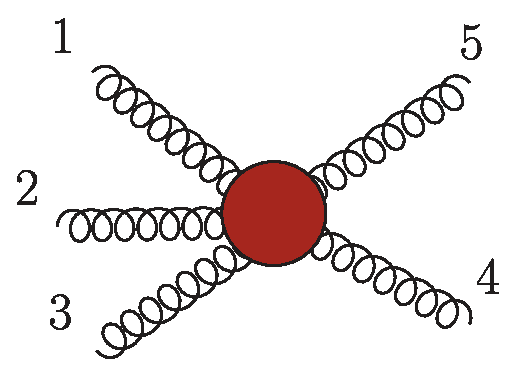
\includegraphics[height=\figureheight]{TreeFull}}} 
    \qquad \xrightarrow[p^2_\xi \to m_\xi^2]{} \quad
    \frac{1}{p^2_\xi - m_\xi^2} \cdot
    \sum_{i\in \text{states}}^{} ~
    \vcenter{\hbox{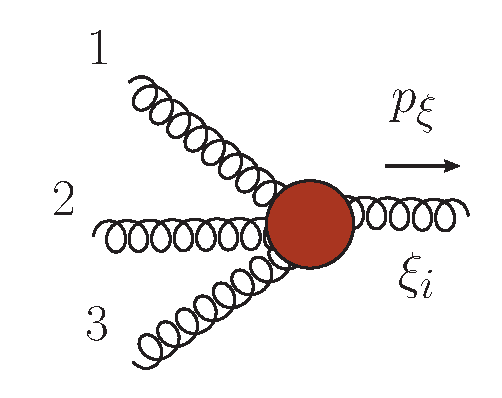
\includegraphics[height=0.9\figureheight]{TreeLeft}}}\cdot
    \vcenter{\hbox{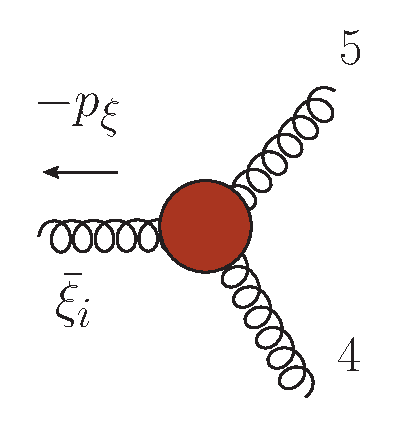
\includegraphics[height=0.9\figureheight]{TreeRight}}}
  \end{equation*}
  \caption{
    An example of factorization due to a physical pole singularity. 
    Here $p_\xi =  p_1 + p_2 + p_3$.
  }
  \label{fig:factorization}
\end{figure}


The exact singularity as expected cannot be reached in any physical process.
However if we analytically continue an amplitude to complex external momenta,
it is possible to choose them to hit the pole explicitly
while still satisfying on-shell conditions for external states.


\subsection{On-Shell Recursion}
\label{sec:BCFW}

The universal factorization  property expressed by \cref{eq:factorization_pole} is independent of perturbation theory. 
For tree-level amplitudes however the factorization can be discovered rather straightforwardly by inspection,
although it might be obscured in the expressions found within the standard Feynman-diagrammatic approach.

The factorization of tree amplitudes can be converted into an algorithm to evaluate them.
This is done through the systematic exploration of the amplitude's factorization limits such that
it can be broken down recursively to sums of lower-multiplicity tree amplitudes. 
The building blocks of this recursion are thus on-shell amplitudes.
This idea is known as \emph{Britto-Cachazo-Feng-Witten} (BCFW) recursion \cite{Britto2005c,Britto2005f}.
The on-shell recursion is a very powerful tool for analytical computations, especially 
in theories with supersymmetry \cite{Dixon:2010ik,Drummond:2008cr,Bourjaily:2010wh}.
However for numerical applications and general models the on-shell recursion algorithm
does not offer benefits over off-shell alternatives, both in speed and numerical stability \cite{Duhr:2006iq,Drummond:2008cr,Badger:2012uz},
especially if one is interested in tree amplitudes in arbitrary number of space-time dimensions (see \cref{chap:numunitarity}). 


\subsection{Generalized Cuts}

Unitarity can be turned into a computational method of loop amplitudes as well.
A certain class of one-loop amplitudes, which
can be written as a sum of box, triangle, and bubble scalar integrals,
\begin{equation} \label{eq:cut_constructable_ampl}
  A^{(1)} = \sum_i d_{i}\,\vcenter{\hbox{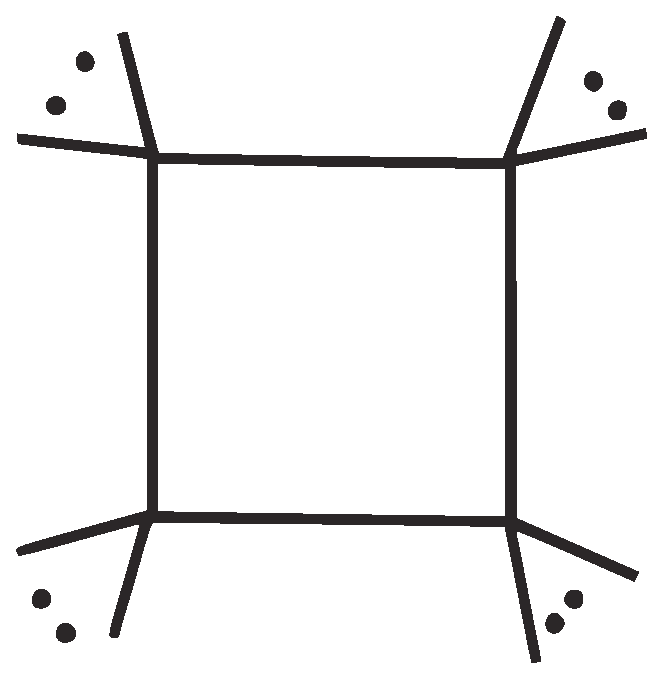
\includegraphics[width=8ex]{boxintegral}}}_i~+~
  \sum_{i}^{} c_{i}\,\vcenter{\hbox{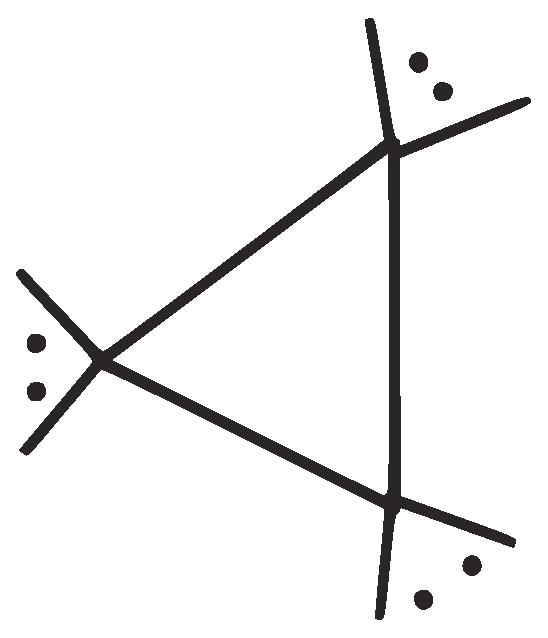
\includegraphics[width=7ex]{triangleint}}}_i~+~
  \sum_i b_{i}\,\vcenter{\hbox{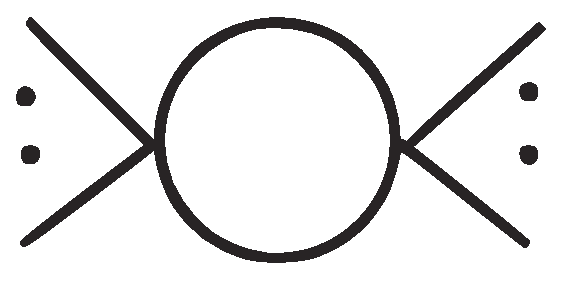
\includegraphics[width=8ex]{bubint}}}_i
\end{equation}
can be obtained entirely from unitarity cuts computed through Cutkosky rules \cite{Bern:1994cg,Bern:1994zx}.
Each integral in \cref{eq:cut_constructable_ampl} has unique discontinuities.
So the discontinuities of the loop amplitude on the left, 
evaluated as phase-space integrals over products of on-shell tree amplitudes as follows from unitarity,
can be matched to those of integrals to obtain equations for the integral coefficients.
However, in general, \emph{only} unitarity is not enough to obtain the full amplitude.

It is possible to generalize application of cuts given by \cref{eq:cut} to
obtain multi-channel discontinuities \cite{Britto:2004nc}.
For example see \cref{fig:quad_cut}.
Note that this kind of cuts are not direct consequences of unitarity of the $\mathcal{S}$-matrix (\cref{eq:unitarity_smatrix}), hence the name \emph{generalized} cuts.

\begin{figure}[ht]
  \centering
  \begin{equation*}
    \vcenter{\hbox{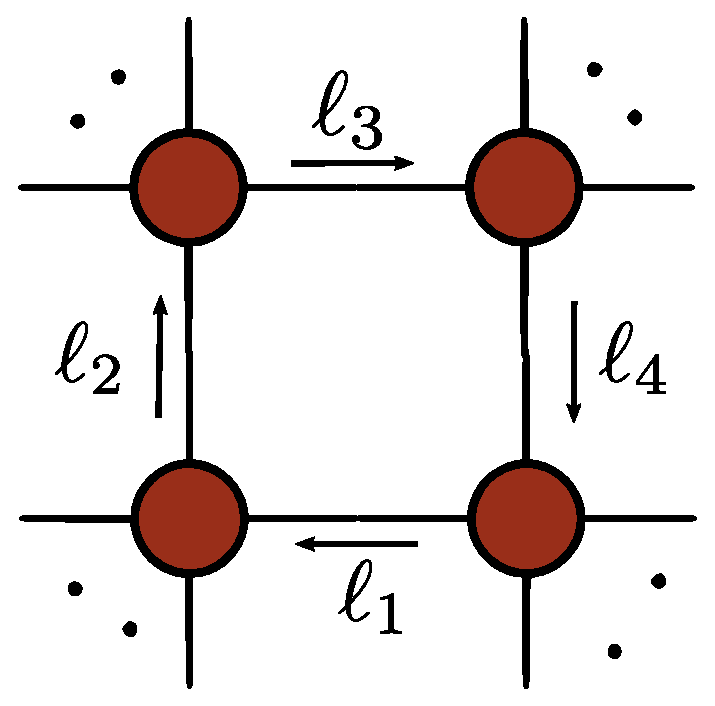
\includegraphics[width=0.2\linewidth]{box}}} \qquad \xrightarrow[i\in\{1\ldots4\}]{\ell_{i}^2-m_i^2\to~0} \qquad
    \vcenter{\hbox{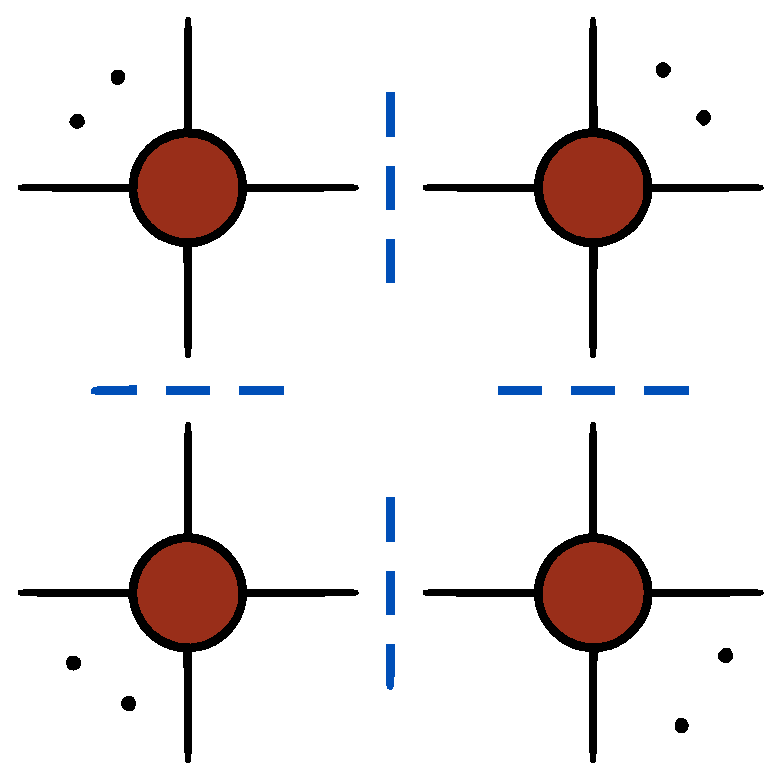
\includegraphics[width=0.2\linewidth]{boxCut}}}
    \quad = \quad \sum_{i}  c_{i} ~ m_{i}(\ell) %+ \sum_{i}  \tilde{c}_{i} \,\tilde{m}_{i}(\ell)
  \end{equation*}
  \caption{
    An example of a generalized cut.
    The loop momentum is chosen such that four propagator are simultaneously put to zero.
    On the left \emph{all} diagrams with the chosen propagators contribute.
    In the factorization limit each corner is a tree amplitude.
    The cut is matched to a basis of loop-momentum polynomials $\{m_i(\ell)\}$ on the right.
  }
  \label{fig:quad_cut}
\end{figure}


As a next step one can use the factorization of amplitudes on the cuts at the \emph{integrand} level  and match
it to a basis of loop-momentum polynomials in numerators (see \cref{fig:quad_cut}),
instead of integral coefficients \cite{Giele:2008ve,Ellis:2007br,Ellis:2008ir,Berger:2008sj}.
This matching procedure is intimately connected to a purely algebraical method of integral reduction known as OPP \cite{Ossola:2006us}.
This method uses the cut conditions \cref{eq:cut} to set some propagators to zero and triangularize linear systems for determining the basis coefficients.
It can be applied individually to each Feynman diagram or a sum thereof, thus having very little to do with factorization and unitarity.
The flexibility and efficiency of the OPP reduction allows a straightforward automation of the computation of generic one-loop amplitudes
(see e.g.\ \cite{Berger:2008ag,Berger:2008sj,Cullen:2011ac,Mastrolia:2010nb,Ossola:2007ax}).

Most of the ideas mentioned in this section are formulated in the context of one-loop computations.
Going beyond one-loop, many of them do not generalize straightforwardly, and require much more sophisticated computational techniques,
which we consider in \cref{chap:numunitarity}.
